\documentclass[a4paper]{article}

\usepackage{calc}
\setlength\textwidth{7in}
\setlength\textheight{10in}
\setlength\oddsidemargin{(\paperwidth-\textwidth)/2 - 1in}
\setlength\topmargin{(\paperheight-\textheight
-\headheight-\headsep-\footskip)/2 - 1in}

%sinuit
\usepackage{siunitx}
%image insertion
\usepackage{graphicx} %image settings
\DeclareGraphicsExtensions{.pdf,.png,.jpg}

%math
\usepackage{amsmath} %math
%\usepackage{cmbright} %math font

%font
\usepackage{kotex}
\usepackage{fontspec}
\ifx가가
\setmainhangulfont[Ligatures=TeX,
BoldFont={KoPubBatang Medium}]{KoPubBatang Light}
\setsanshangulfont[Ligatures=TeX,
BoldFont={KoPubDotum Medium}]{KoPubDotum Light}
\setmainhanjafont[Ligatures=TeX,
BoldFont={KoPubBatang Medium}]{KoPubBatang Light}
\setsanshanjafont[Ligatures=TeX,
BoldFont={KoPubDotum Medium}]{KoPubDotum Light}
\xetexkofontregime[puncts=prevfont, colons=prevfont, cjksymbols=hangul]{latin}
\fi

%줄간격
\usepackage{setspace}
%\usepackage{indentfirst}
\setstretch{1.2}
\everydisplay{\setstretch{1.2}}

%subfigure
\usepackage{subfigure}

\pagestyle{plain}
\title{물리 실험보고서 1}
\author{이한빈, 의예과 2016-13347}

\begin{document}


\numberwithin{equation}{section}
\maketitle

\section{Introduction}
	폐회로가 주어졌을 때 회로 내부를 지나가는 자기선속이 변하면 크기는 시간당 변화량에 비례하며 방향은 자기선속 변화의 반대인 기전력이 회로에 유도된다.
	이를 페러데이의 법칙이라고 하며 다음과 같이 표현된다.
	\begin{equation} \label{faraday}
		\epsilon = -\frac{d\Phi}{dt} 
	\end{equation}
	여기서 기전력의 방향이 자기선속 변화의 반대라는 사실을 렌츠의 법칙이라고 부른다.

	페러데이의 법칙을 이용하면 그림과 같은 전동기에서 발생하는 기전력을 계산할 수 있다.
	회로의 면적을 $A$, 회전각속력을 $\omega$, 회로가 놓여진 공간의 자기장을 $B$라고 하자.
	\begin{figure}[h] 
		\centering 
		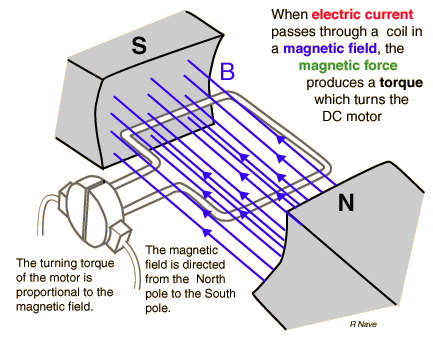
\includegraphics[width=0.4\textwidth]{img/motor.png}
		\caption{전동기}
		\label{fig:motor}
	\end{figure}
	처음에 자기장과 면벡터가 나란하면 시간에 따른 자기선속은 다음과 같다.
	\begin{equation} \label{line}
		\Phi = \vec{A} \cdot \vec{B} = AB\cos{}\omega{}t
	\end{equation} 

	식 (\ref{faraday})과 식 (\ref{line})으로부터 전동기에서 발생하는 기전력을 구하면 다음과 같다.
	\begin{equation}
		\epsilon = -\frac{d\Phi}{dt} = AB\omega{}\sin{}\omega{}t
		\label{eq:period}
	\end{equation}

	따라서 일정한 속력으로 회전하는 전동기에서 발생하는 기전력은 사인파의 형태로 나타남을 알 수 있다.
	반대로 전류가 흐르는 폐회로는 자기장에서 토크를 받는다.
	장치가 전동기와 동일하게 되어있다고 가정하고 회로에 전류 $I$가 흐른다고 하자.
	회로의 자기모멘트는 다음으로 주어진다.
	\begin{equation}
		\vec{\mu} = I\vec{A}
	\end{equation}

	회로가 받는 토크는 자기모멘트와 자기장의 외적이므로 폐회로가 받는 토크는 다음과 같다.
	\begin{equation}
		|\vec{\tau}| = |\vec{\mu} \times \vec{B}| = IAB\sin{\omega{}t}
		\label{eq:error}
	\end{equation}

 	전동기에서 직류전원을 연결하면 식 (\ref{eq:error})에서 볼 수 있듯이 전동기가 지속적으로 같은 방향으로 회전하지 않고 진동하는 것을 알 수 있다.
 	이를 극복하기 위해 회로에 흐르는 전류의 방향을 지속적으로 바꾸는 장치를 정류자라고 한다.
 	\begin{figure}[h]   		
 		\centering
 		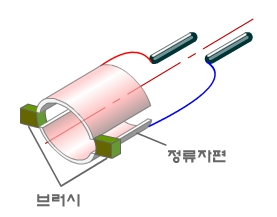
\includegraphics[scale=0.5]{img/a-5385.jpg}
 		\caption{2단 정류자}
   		\label{fig:com}
 	\end{figure}

 	그림 \ref{fig:com}의 정류자는 전류의 방향이 $\ang{180;;}$마다 역전되므로 회로가 받는 토크는 원래토크에서 절댓값이 씌어진 형태가 된다.
 	기전력이 유도되는 상황에서도 마찬가지로 기전력은 절댓값이 씌어진 다음과 같은 형태로 주어진다.
 	\begin{equation}
 		|\epsilon| = AB\omega{}|\sin{\omega t}|
 		\label{eq:commnute}
 	\end{equation}

 	본 실험에서는 첫 번째로 솔레노이드와 막대자석을 이용하여 렌츠의 법칙을 검증한다.
 	두 번째로는 전동기에 연결된 회로를 균일한 자기장 속에서 회전 시켰을 때 유도되는 기전력을 측정하여 렌츠의 법칙과 페러데이의 법칙을 검증한다.
 	또 전동기의 AC, DC출력 단자에 대해 각각 실험하고 비교함으로써 정류자의 효과에 대해서도 알아봤다.

	\section{Method}
	\subsection{렌츠의 법칙 확인}
	준비물 : 막대자석, 솔레노이드, 오실로스코프
	솔레노이드의 양 극을 오실로스코프에 연결했다. 
	그 후 N극을 솔레노이드 내부에 넣은 상태로 당길 때 오실로스코프로 측정된 기전력의 방향을 얻었다.
	당기는 대신 N극을 넣을 때 오실로스코프로 측정한 기전력의 방향을 얻었다.
	위 과정을 N극 대신 S극으로 반복했다.

	\begin{figure}[h]
		\centering
		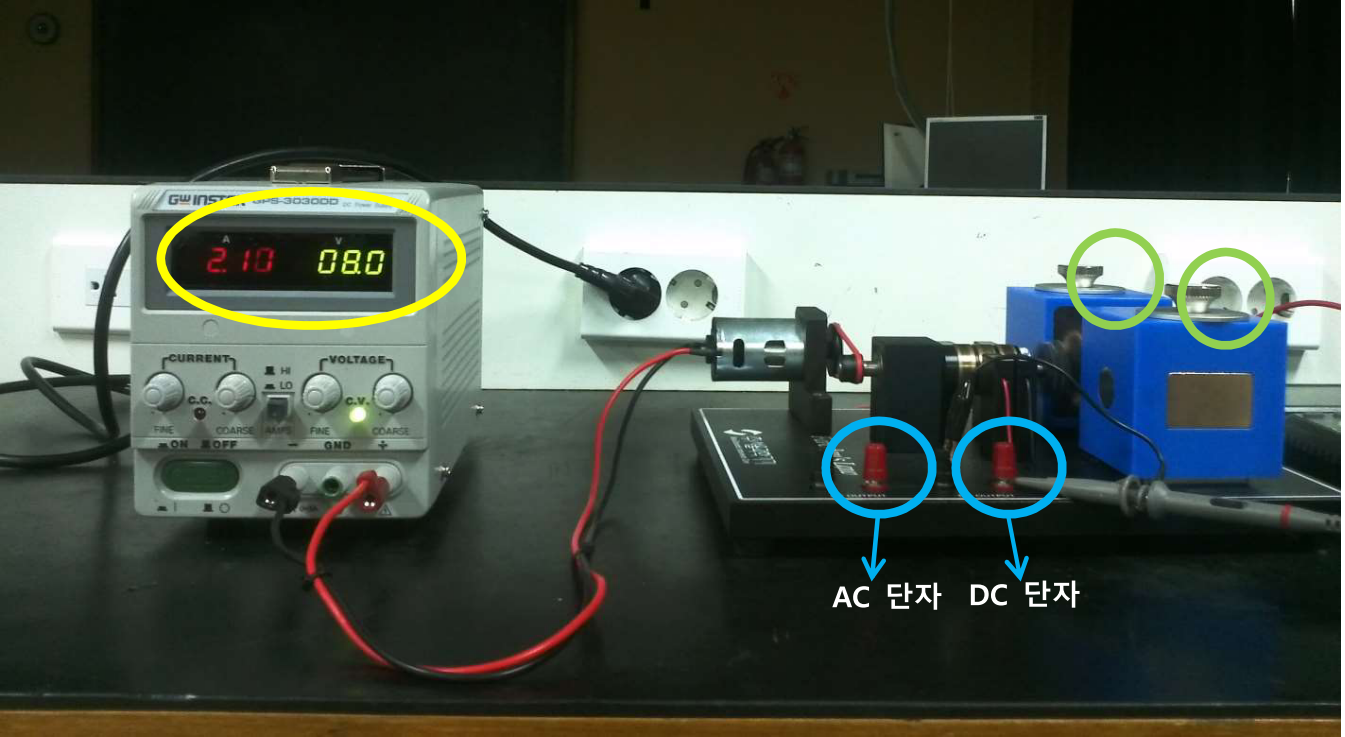
\includegraphics[width=0.7\textwidth]{img/exp1.PNG}
		\label{fig:exp1}
		\caption{오른쪽 : Faraday 실험장치, 왼쪽 : 직류전원장치}
	\end{figure}

	\subsection{Faraday 실험장치 DC 출력 기전력 측정}
	준비물: Faraday 실험장치, 전동기, 직류전원장치
	오실로스코프를 Faraday 실험장치의 DC단자에 연결했다.
	직류전원장치를 Faraday 실험장치에 연결하고 직류전원장치의 전류와 전압 그리고 자석을 표 \ref{tb:dctable}같이 설정했다.
	각 설정마다 오실로스코프로 시간에 따른 기전력 변화를 측정했다.
	
	\subsection{Faraday 실험장치 AC 출력 기전력 측정}
	준비물: Faraday 실험장치, 전동기, 직류전원장치
	오실로스코프를 Faraday 실험장치의 AC단자에 연결했다.
	직류전원장치를 Faraday 실험장치에 연결하고 직류전원장치의 전류와 전압 그리고 자석을 표 \ref{tb:actable}같이 설정했다.
	각 설정마다 오실로스코프로 시간에 따른 기전력 변화를 측정했다.
	
	\begin{figure}[h]
		\centering
			\subfigure[DC 출력]{
			\begin{tabular}{cc}
				\hline \hline
				전류 & 전압 \\
				\hline
				\multicolumn{2}{c}{R=1\si{cm} 원형 자석} \\
				\hline
				2.35A & 9.10V \\
				\hline
				2.20A & 8.00V \\
				\hline
        		\multicolumn{2}{c}{4$\times$2.5\si{cm^2} 직사각형 자석} \\
				\hline
				2.20A & 8.00V \\
				\hline
				2.38A & 9.50V \\
				\hline
				\multicolumn{2}{r}{6$\times$6\si{cm^2} 직사각형 자석} \\
				\hline
				2.30A & 8.60V \\
				2.39A & 9.79V \\
				\hline \hline
			\end{tabular} \label{tb:dctable}
			}
			\quad
			\subfigure[AC 출력]{
			\begin{tabular}{cc}
				\hline \hline
				전류 & 전압 \\
				\hline
				\multicolumn{2}{c}{R=1\si{cm} 원형 자석} \\
				\hline
				2.34A & 9.90V \\
				\hline
				2.42A & 11.00V \\
				\hline
        		\multicolumn{2}{c}{4$\times$2.5\si{cm^2} 직사각형 자석} \\
				\hline
				2.38A & 10.30V \\
				\hline
				2.48A & 12.00V \\
				\hline
				\multicolumn{2}{r}{6$\times$6\si{cm^2} 직사각형 자석} \\
				\hline
				2.36A & 9.80V \\
				2.31A & 9.50V \\
				\hline \hline
			\end{tabular}  \label{tb:actable}
			}
		\caption{실험구성}
	\end{figure}

	\section{Result}
	\subsection{렌츠의 법칙 확인}
		\begin{figure}[h]
			\centering
			\subfigure[N극 넣을 때]{
			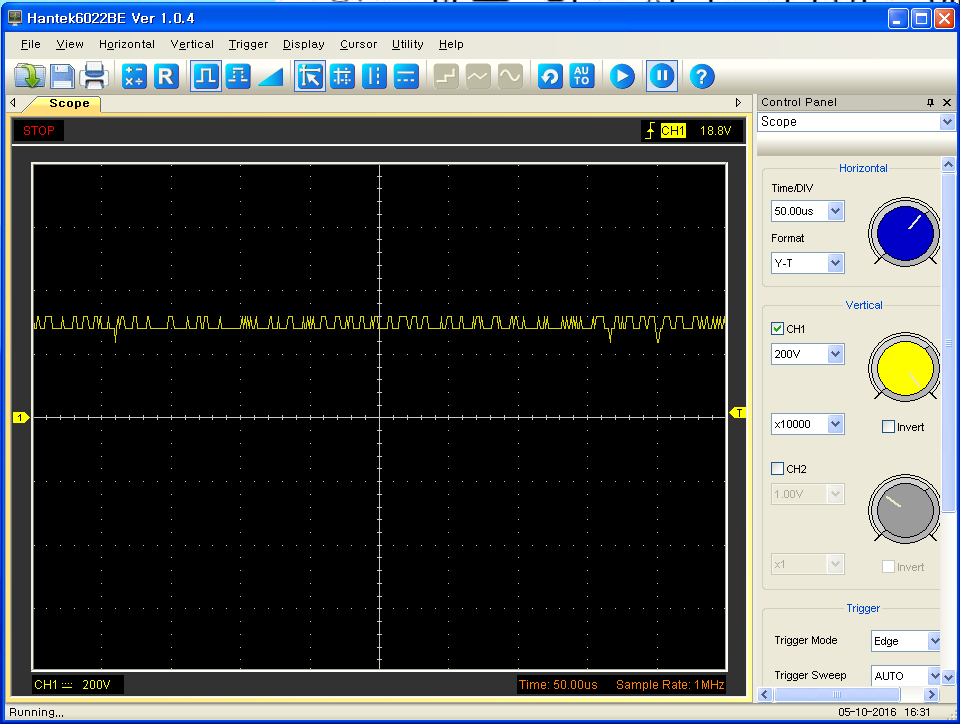
\includegraphics[width=0.22\textwidth]{img/nin.png}
			}
			\subfigure[N극 당길 때]{
			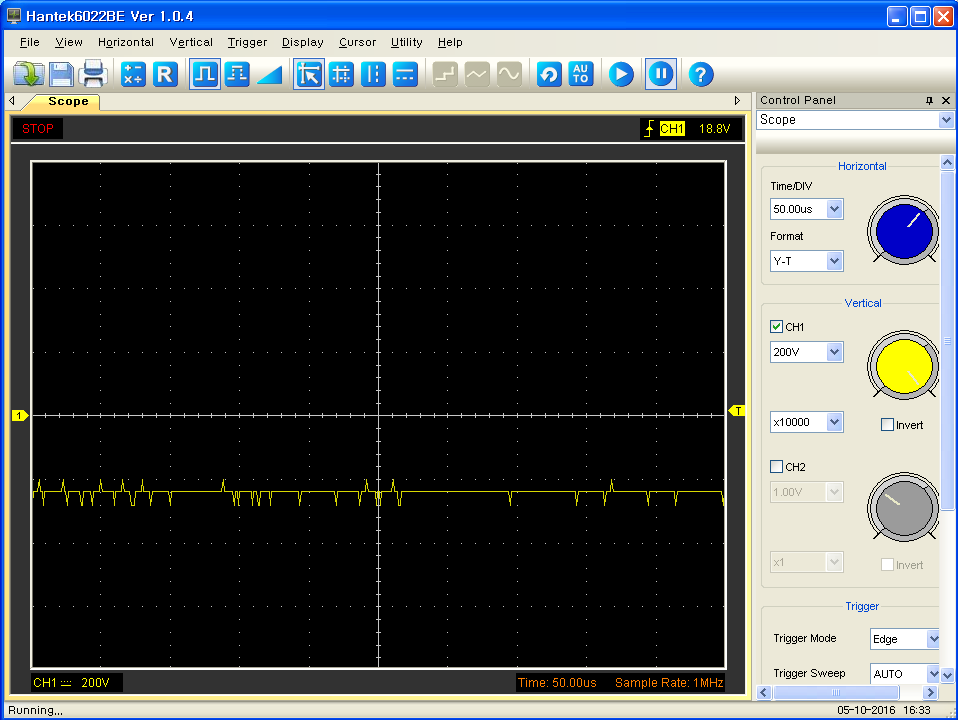
\includegraphics[width=0.22\textwidth]{img/nout.png}
			}
			\subfigure[S극 넣을 때]{
			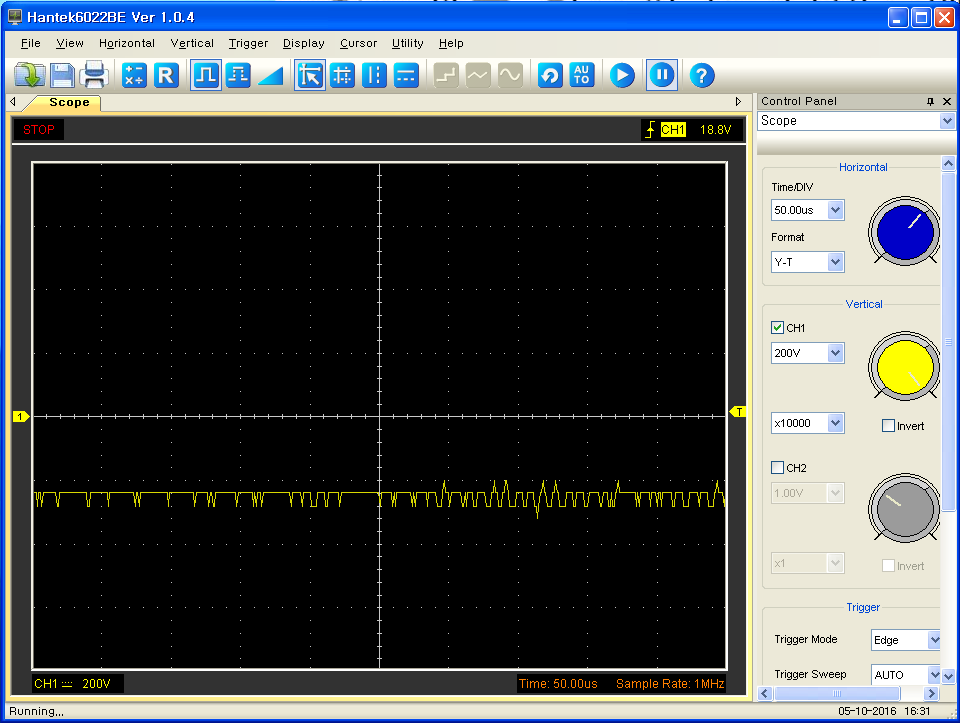
\includegraphics[width=0.22\textwidth]{img/sin.png}
			}
			\subfigure[S극 당길 때]{
			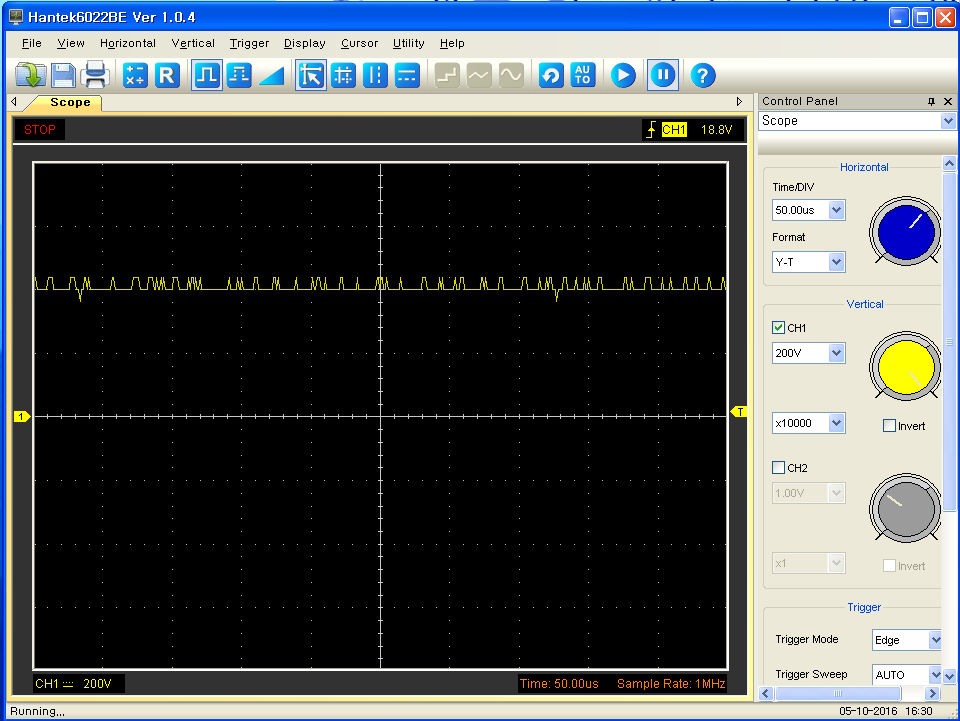
\includegraphics[width=0.22\textwidth]{img/sout.png}
			}
			\caption{렌츠의 법칙 확인 실험} \label{fig:lentz}
		\end{figure}
	솔레노이드는 +극쪽으로 봤을 때 시계방향으로 감겨있었다. 그림(\ref{fig:lentz})에서 양의 값은 +극에서 -방향의 기전력을 뜻한다. (a)결과를 보면 N극이 솔레노이드에 접근하면 (+)방향으로 기전력이 발생한 것을 볼 수 있다. (b),(c),(d)에서는 자석의 극성과 움직이는 방향이 반대로 바뀔 때마다 기전력의 부호가 (a)와 반대로 바뀌는 것을 볼 수 있다.

\newpage
	실험 3.2와 3.3에서는 파일에 기록된 측정간 시간 간격(10$\si{ms}$)에 실험횟수($>10^6$)을 곱했을 때 전동기의 회전주기가 모두 500초가 넘었는데 이는 프로그램 오류로 보인다.
	따라서 주기는 알 수 없고 기전력의 진폭만 알 수 있다.
	Y축은 기전력, X축은 시간에 따라 측정된 값의 횟수이다. 
	\subsection{Faraday 실험장치 DC 출력 기전력 측정}
	\begin{figure}[h]
		\centering
		\subfigure[2.35A 9.10V]{
		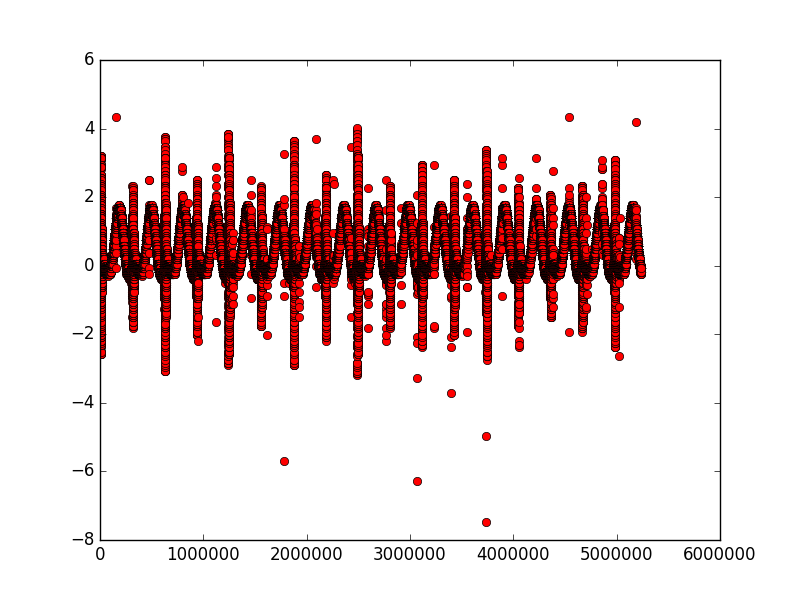
\includegraphics[width=0.25\textwidth]{img/DC/2.36_9.11st.png}
		}
		\subfigure[2.20A 8.00V]{
		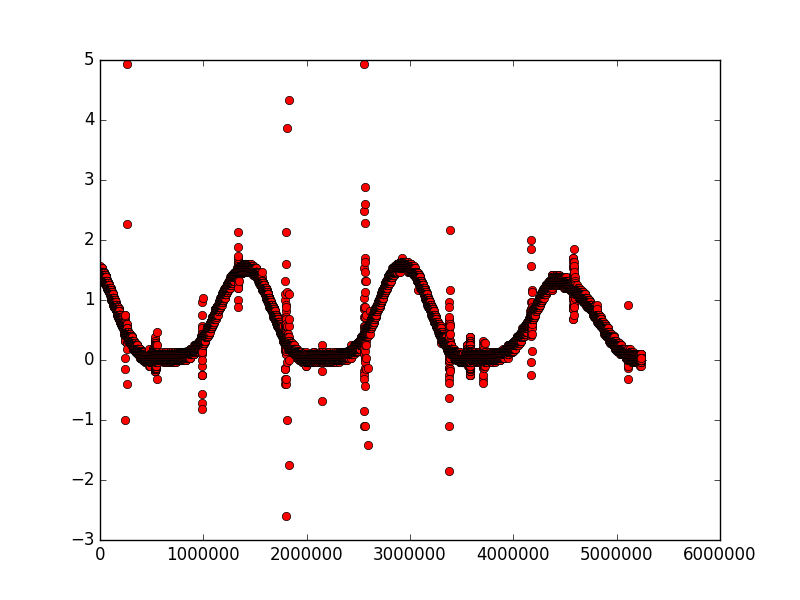
\includegraphics[width=0.25\textwidth]{img/DC/2.2_83rd.png}
		}
		\subfigure[2.30A 8.60V]{
		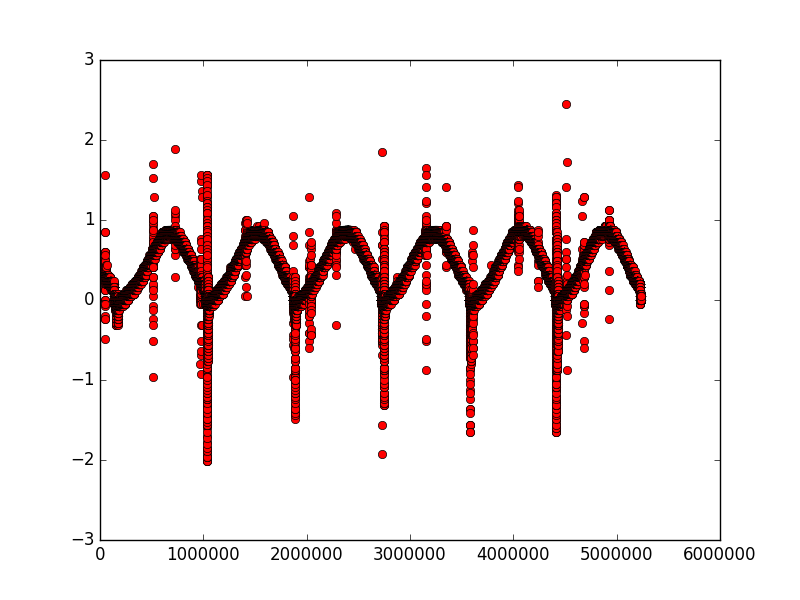
\includegraphics[width=0.25\textwidth]{img/DC/2.3_8.65th.png}
		}
		\\
		\subfigure[2.20A 8.00V]{
		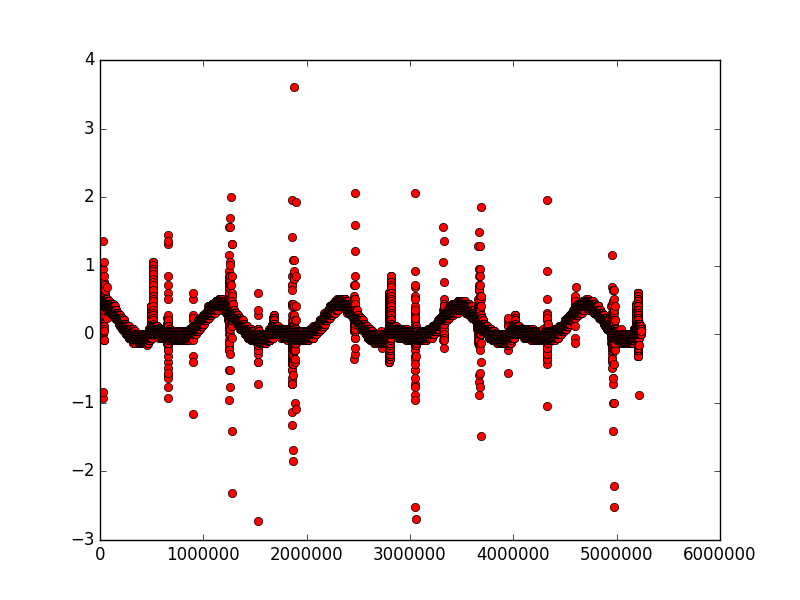
\includegraphics[width=0.25\textwidth]{img/DC/2.3_82nd.png}
		}
		\subfigure[2.38A 9.50V]{
		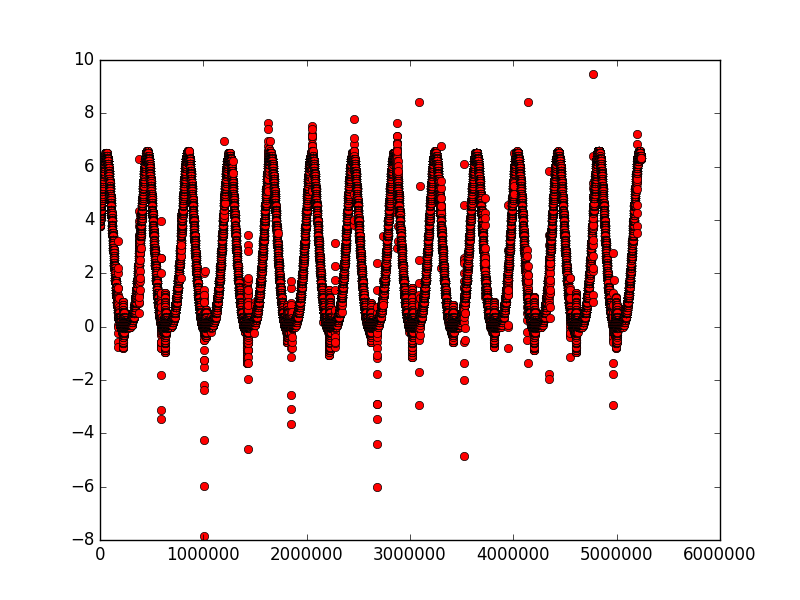
\includegraphics[width=0.25\textwidth]{img/DC/2.38_9.54th.png}
		}
		\subfigure[2.39A 9.79V]{
		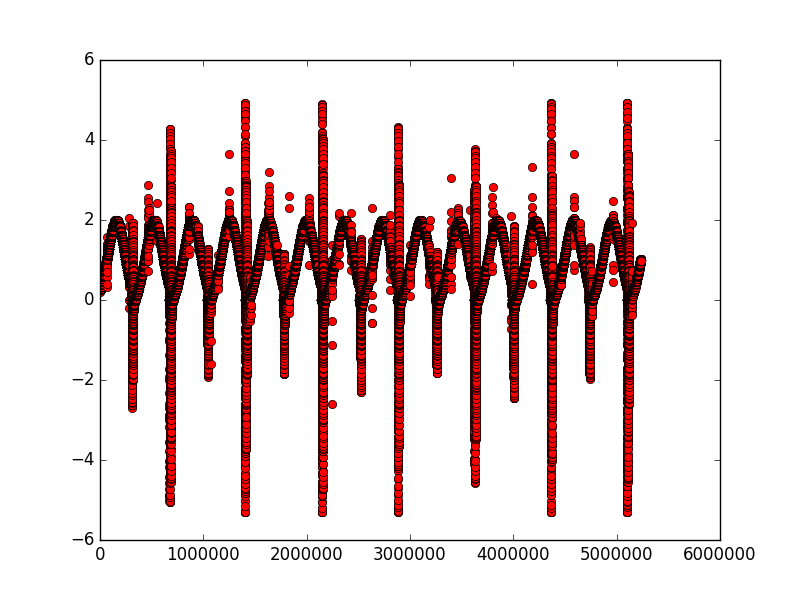
\includegraphics[width=0.25\textwidth]{img/DC/2.37_9.76th.png}
		}
		\caption{DC 출력, 자석의 크기는 1열:R=1\si{cm} 2열:4$\times$2.5\si{cm^2} 3열:6$\times$6\si{cm^2}}
	\end{figure}
	측정값들이 모두 양의 값만 가지며 주기적으로 진동한다.
	인가되는 전압과 전류가 커질 수록 유도기전력의 진폭이 커짐을 알 수 있다.
	자석이 커질 수록 유도기전력의 세기도 커진다.
	

	\subsection{Faraday 실험장치 AC 출력 기전력 측정}
	\begin{figure}[h]
		\centering
		\subfigure[2.34A 9.90V]{
		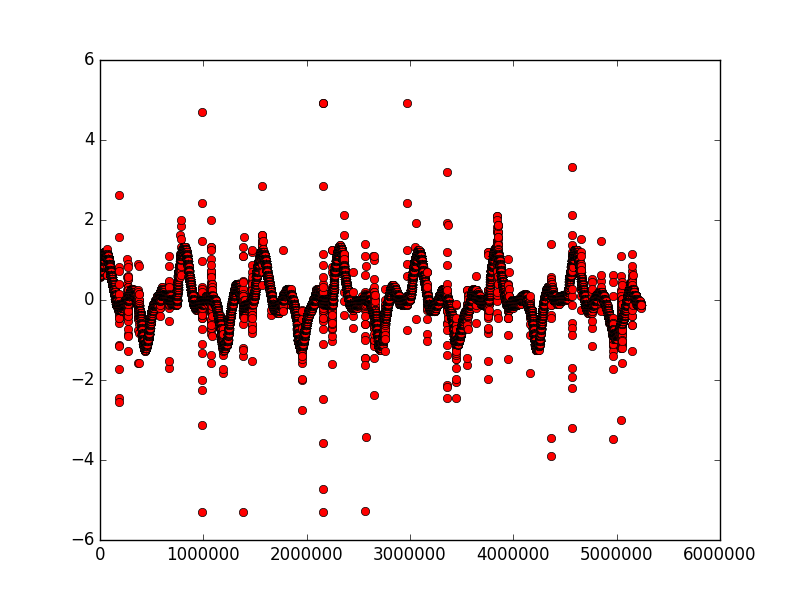
\includegraphics[width=0.25\textwidth]{img/AC/2.34_9.95th.png}
		}
		\subfigure[2.38A 10.30V]{
		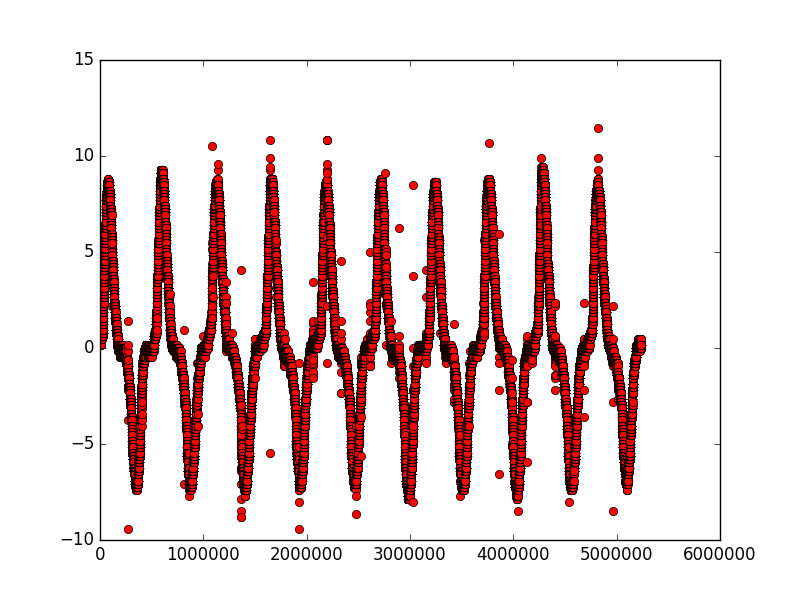
\includegraphics[width=0.25\textwidth]{img/AC/2.38_10.33rd.png}
		}
		\subfigure[2.36A 9.80V]{
		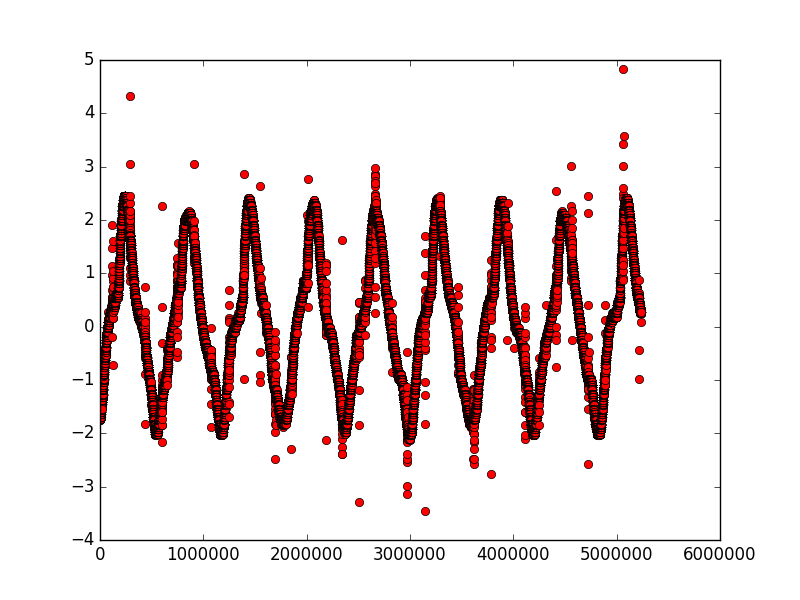
\includegraphics[width=0.25\textwidth]{img/AC/2.36_9.81st.png}
		}
		\\
		\subfigure[2.42A 11.00V]{
		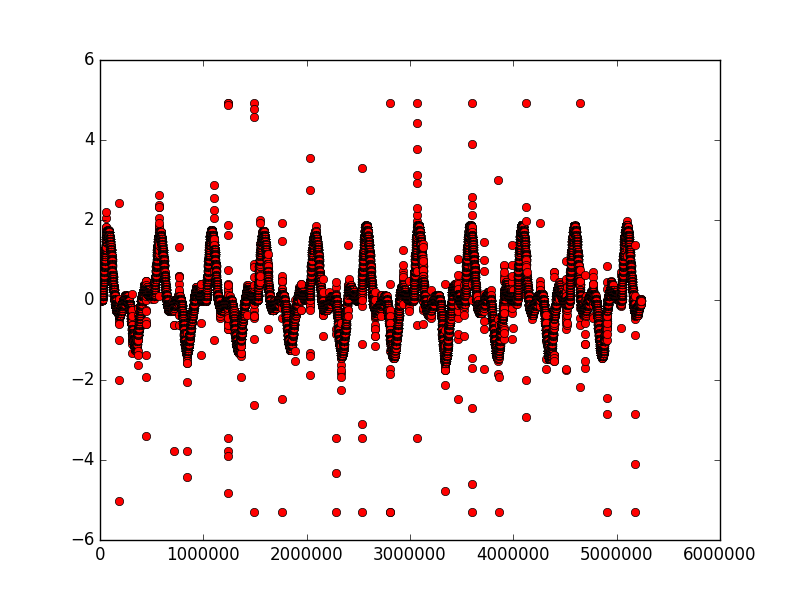
\includegraphics[width=0.25\textwidth]{img/AC/2.41_116th.png}
		}
		\subfigure[2.48A 12.00V]{
		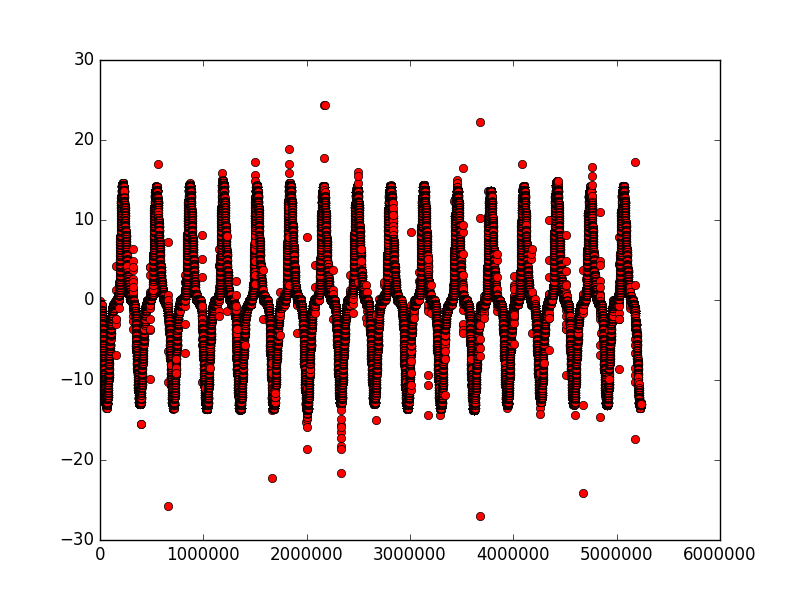
\includegraphics[width=0.25\textwidth]{img/AC/2.48_124th.png}
		}
		\subfigure[2.31A 9.50V]{
		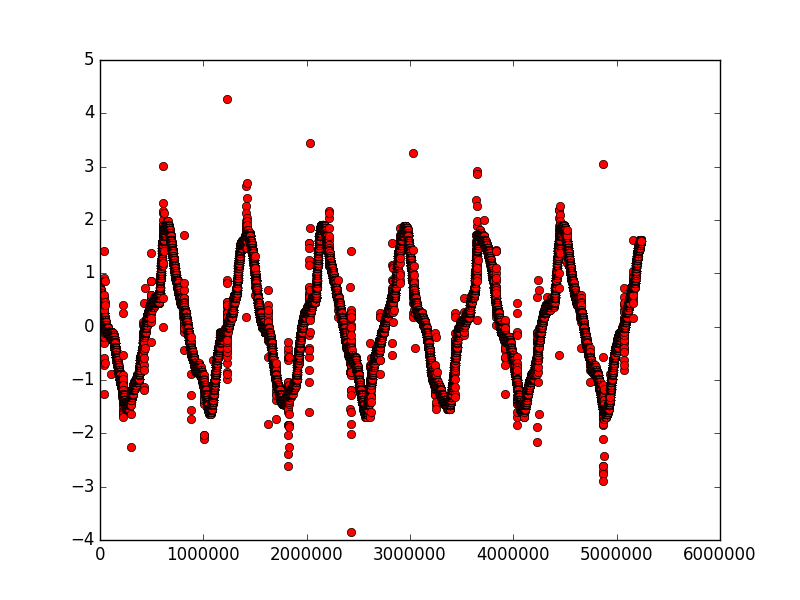
\includegraphics[width=0.25\textwidth]{img/AC/2.31_9.5.png}
		}
		\caption{AC 출력, 자석의 크기는 1열:R=1\si{cm} 2열:4$\times$2.5\si{cm^2} 3열:6$\times$6\si{cm^2}}
	\end{figure}
	측정값들이 주기적으로 진동하며 인가되는 전압과 전류가 커질 수록 유도기전력의 진폭이 커짐을 알 수 있다. 자석이 커질 수록 유도기전력의 세기도 커진다.

	\newpage

	\section{Conclusion}
	첫 번째 실험에서는 렌츠의 법칙을 확인할 수 있었다. 
	그림 (\ref{fig:lentz})의 (a)에 나타난 기전력의 방향을 보면 N극이 다가오는 방향으로 솔레노이드가 N극을 띤 것을 알 수 있다(오른손 법칙). 
	이는 자기선속의 변화에 저항하는 방향으로 자기장을 형성하도록 솔레노이드에 기전력이 유도된다는 렌츠의 법칙과 일치한다. 
	자석의 극성과 자석이 움직인 방향이 바뀔 때마다 기전력의 부호가 역전된다는 것을 보여준 나머지 결과들도 렌츠의 법칙과 잘 일치한다.

	AC, DC단자로 실험한 모든 결과들에서 기전력은 시간에 따라 진동하는 것으로 나타났다. 
	이는 기전력이 주기적으로 진동한다고 예측한 식 (\ref{eq:period})과 잘 일치한다.

	하지만 실험결과들은 식 (\ref{eq:period})과는 다르게 매끄러운 삼각함수이 아니었다.
	실험결과에서 다른 점들과 크게 벗어나는 점들은 비교적 균일한 분포를 가지고 있으며 오실로스코프에 아무런 입력이 없을 때도 계속 나타났었다.
	따라서 앞서 언급한 점들의 오차는 랜덤한 노이즈로 볼 수 있다.
	오실로스코프에 랜덤한 노이즈가 유입되고 있거나 전동기에 마찰 등을 원인으로 추정해볼 수 있다.
	그러나 실험결과가 삼각함수와 다른 주기함수를 띠는 것은 주기적으로 나타나는 오차요인이 존재함을 시사한다.
	Reference에 첨부된 코드로 FT(푸리에변환)을 시행하면 위상만 다르고 진동수는 같고 위상이 다른 파동이 크게 두 개가 나타난다.
	제일 큰 파동의 경우 식 (\ref{eq:period})이 예측한 회전에 의한 유도기전력으로 볼 수 있다.
	두 번째로 큰 파동은 식 (\ref{eq:error})로 인해 생긴 토크로 $\omega$가 바뀌면서 생긴 것으로 볼 수 있다. 왜냐하면 토크의 바뀌는 주기가 회전이 바뀌는 주기와 일치하기 떄문이다.
	
	DC단자로 실험한 결과들을 보면 기전력이 (-)부호를 갖지 않는 것을 볼 수 있다.
	AC단자로 실험한 결과들과 비교해보면 (-)부호를 가져야할 부분들이 (+)부분들로 올라온 것으로 볼 수 있다.
	이는 정류자가 장착된 경우 기전력 그래프가 정류자가 없는 경우와 절댓값 함수의 합성으로 나타난다는 식 (\ref{eq:commnute})의 예측과 잘 일치한다.	

	마지막으로 자석의 크기가 클수록 전동기에 인가된 전류와 전압이 클수록 유도기전력의 크기가 커짐을 알 수 있었다. 전동기에 인가된 전류와 전압이 클수록 회전 속도가 빨라진다는 사실로부터 이 결과가 식 (\ref{eq:period})와 잘 일치함을 알 수 있다.  



\section{Reference 및 부록}
	1. Halliday, D., Resnick, R., \& Walker, J. (2014). {\it{}Principles of Physics} (10th ed., Vol. 2). Hoboken, NJ: Wiley.
	\\ 
	2. FFT Code http://pastebin.com/8g6wAP03

\end{document} 

%실험에서 개선할 점 등 피피티에서 봤던 거 모두 적어서 처리합시다